\begin{figure*}[ht!]
\centering
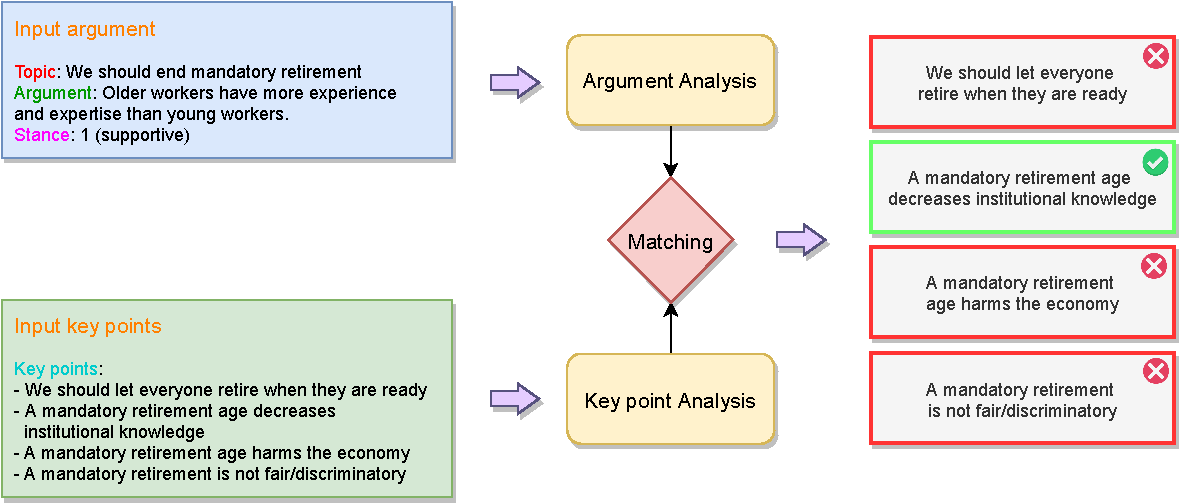
\includegraphics[scale=0.74]{figures/KPA-workflow.pdf}
\caption{Overview of the Key Point Matching workflow in the Quantitative Summarization – Key Point Analysis Shared Task Track 1. From the information retrieval perspective, this task is to identify the most salient point that reinforces a given query.}
\label{fig:workflow}
\end{figure*}


\begin{abstract}
Key Point Analysis (KPA) is one of the most essential tasks in building an Opinion Summarization system, which is capable of generating key points for a collection of arguments toward a particular topic. Furthermore, KPA allows quantifying the coverage of each summary by counting its matched arguments. With the aim of creating high-quality summaries, it is necessary to have an in-depth understanding of each individual argument as well as its universal semantic in a specified context. In this paper, we introduce a promising model, named Matching the Statements (MTS) that incorporates the discussed topic information into arguments/key points comprehension to fully understand their meanings, thus accurately performing ranking and retrieving best-match key points for an input argument. Our approach\footnote{The code is available at: \url{https://github.com/VietHoang1512/KPA}} has achieved the $4^{th}$ place in Track 1 of the Quantitative Summarization – Key Point Analysis Shared Task by IBM, yielding a competitive performance of $0.8956\:(3^{rd})$ and $0.9632\:(7^{th})$ strict and relaxed mean Average Precision, respectively.
\end{abstract}

\section{Introduction}
\label{sec:intro}

Prior work in Opinion Summarization often followed the extractive strategy, which identifies the most representative pieces of information from the source text and copies them verbatim to serve as summaries \citep{angelidis-lapata-2018-summarizing, brazinskas2019unsupervised}. Abstractive summarization is a less popular strategy compared to the previous one yet offers more coherent output texts. Approaches governed by this vein could generate new phrases, sentences or even paragraphs that may not appear in the input documents \citep{ganesan-etal-2010-opinosis, isonuma2021unsupervised}. Both extractive and abstractive methods are the straightforward applications of multi-document summarization \citep{liu2018generating, fabbri-etal-2019-multi}, which has been an emerging research domain of natural language processing in recent years.

As is well known, in traditional multi-document summarization methods, the role of an individual or a subset of key points among the summaries is often neglected. To be more specific, \citet{bar-haim-etal-2020-arguments} posed a question regarding the summarized ability of a small group of key points, and to some extent answered that question on their own by developing baseline models that could produce a concise bullet-like summary for the crowd-contributed arguments.
With a pre-defined list of summaries, this task is known as Key Point Matching (KPM). Figure \ref{fig:workflow} provides a simple illustration of the KPM problem, where the most relevant key points are retrieved for each given argument within a certain topic (i.e. context).

Inspired by the previous work that studied the problem of learning sentence representation \citep{cer2018universal, reimers-gurevych-2019-sentence} and semantic similarity \citep{yan2021consert}, we propose Matching The Statements (MTS), which further takes the topic information into account and effectively utilizes such proper features to learn a high performance unified model. Our approach has benefited from the recent developments of pre-trained language models such as BERT \citep{devlin2018bert}, ALBERT \citep{lan2019albert} or RoBERTa \citep{liu2019roberta}.

Our contributions in this paper could be depicted as follows:
\begin{itemize}
    \item Firstly, we design a simple yet efficient network architecture to fuse the context into sentence-level representations. Instead of letting the model infer the implicit reasoning structure, we provide our model with the information on whether an argument or key point (which are collectively referred to as statements in the remainder of this paper) supports its main topic or not.
    \item Secondly, our method adopts the pseudo-labels mechanism \citep{ge2020mutual, zhang2021refining}, where we label arguments that belong to the same key point (and the key point itself) by the same index. The goal is to learn an embedding space in which the embedded vectors of mutual supportive statement pairs (i.e. having the same label) are pulled closer whereas unrelated ones are pushed apart. 
    \item Finally, we validate the proposed MTS on the ArgKP-2021 \citep{bar-haim-etal-2020-arguments} dataset in a variety of protocols. Extensive experiment results show that our proposed method strongly outperforms other baselines without using external data, thus becoming a potential method for the Key Point Matching problem.
\end{itemize}

The rest of this paper is organized in the following way: Section \ref{sec:related-work} briefly reviews the related work, while section \ref{sec:problem} formulates the KPM problem. Next, we describe our methodology in section \ref{sec:method}, followed by the experimental results in section \ref{sec:experiment}. Finally, section \ref{sec:conclusion} will conclude our work and discuss future directions for further improvements.

